\documentclass[a4paper]{article}
\usepackage[english]{babel}
\usepackage[utf8]{inputenc}
\usepackage{hyperref}
\usepackage{graphicx}
\usepackage{wrapfig}
\usepackage{listings}
\usepackage{float}
%\usepackage{bytefield}
%\usepackage{fullpage}
%\usepackage{algorithm}
%\usepackage{algpseudocode}
%\usepackage{amsmath}
%\usepackage[colorinlistoftodos]{todonotes}

\title{Timing Analysis Attack Simulation in Tor Networks}

\author{Matteo Martelli, Davide Berardi}

\date{\today}

\begin{document}
\maketitle

\begin{abstract}
In this document we talk about blablabla
\end{abstract}

\section{Introduction}
Protecting data privacy on the Web is a very hot topic nowadays. 
Users of the Web may want to surf without the risk that their personal
informations can be read by other users. %TODO and governal agencies
%that may be also intersted in our data, cite the article about it
One of the most largely-used
architecture for this purpose is the \emph{Onion Routing} and its
protocol implementation: \emph{Tor}\cite{tor}. In fact, the latter is modeled with
several techniques with the aim to provide communication security and
data privacy to its network users. Anyway there have been recent papers
 pointing out the Tor's vulnerabilities. %TODO ref these papers
As the Tor community itself stages, ``Tor does not provide protection
against end-to-end timing attacks''\cite{tor-overview}, thus the
chance for an attacker to eavesdrop a Tor communication traffic and
discover the users involved in it by a
timing analysis is a well known vulnerability of Tor. 

In this kind of analysis, in order to
identify the source of a communication, the attacker should be able to
trace the outgoing traffic and the incoming traffic from both the
entering and exiting node of the communication path.
Clearly a timing analysis is feasible only under a certain amount of
conditions that are often hard to satisfy. As instance, discovering
that a generic user $U$ is connecting to a server $S$ over a Tor
communication may require tracing the traffic of many users in the
network, as the
attacker cannot know which users may be interested in connecting with
$S$. Also, there may be the need of tracing more than just the
interested server because the attacker can find a better time
relation between the user $U$ and another server $S'$ than between $U$
and the interested server $S$, thus the attacker could exclude $U$ to be a possible
connection source for $S$.
In the section
\ref{sec:tor} we will better describe how Tor works and how the
end-to-end timing attack could be performed.

In order to test the feasibility and the parameters involved in
a time analysis attack over the Tor network, we set up a simulation
scenario in which a series of simulation runs have been performed and some interesting
empirical results have been taken out and analyzed.
At the end we will point out how the Tor time analysis vulnerability can be
critical and we will introduce some proposals to enhance Tor with the
view of preventing this kind of attacks. %TODO cite the proposals (one
%of them http://www.ohmygodel.com/publications/usersrouted-ccs13.pdf

%TODO Introduce the simulation work, made to understand how
%much Tor can be vulnerable

\section{Onion Routing and Tor}
\label{sec:tor}
Tor is an implementation of the onion routing architecture model. The
onion routing consists in a technique that provides anonymous
connections over a computer network\cite{or}.
The connections exist in three phases:
\begin{itemize}
	\item \textbf{Connection Setup}: adflkgjdflkg
	\item \textbf{Data Movement}: sfdsgdfgdf
		\begin{figure}[H]
			\centering
			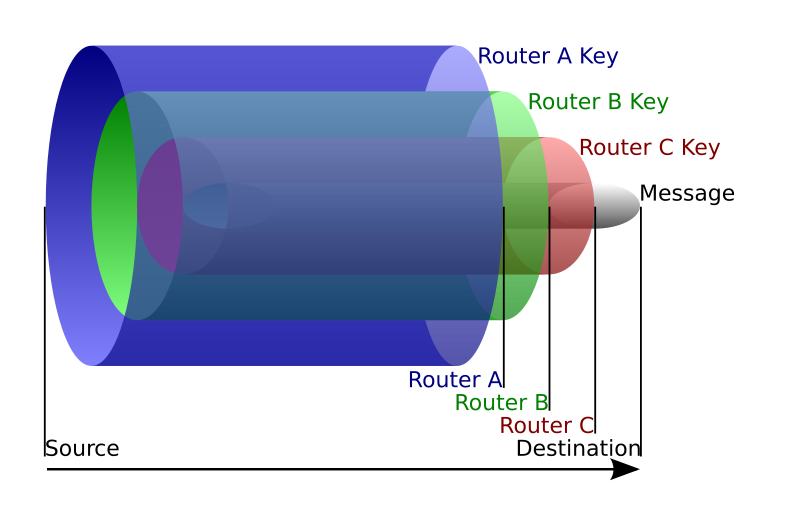
\includegraphics[scale=0.35]{onion.png}
			%TODO\caption{Add caption for this figure}
			\label{fig:onion}
		\end{figure}	
	\item \textbf{Connection Tear-Down}: sdfdjgl
\end{itemize}

\subsection{Tor architecture overview}
%TODO protects you from traffic analysis
%https://www.torproject.org/about/overview.html.en
\subsection{Tor attacks}

\subsection{Timing Attack}

\section{Simulation}
\label{sec:simulation}
\subsection{Shadow}
\subsection{Autosys plugin}
\subsection{Analyzer plugin}
\subsection{Simpletcp plugin}

\section{Data Analysis}
\subsection{Netbuilder Script}
\subsection{Analyzer Script}
\subsection{Empirical Results}

\section{Conclusions}
%TODO: diciamo che effettivamente sembra molto vulnerabile a time
%analysis anche se  si dovrebbe provare con reti più grandi anche se "AS-awareness in Tor
%path selection" dice che non cambia molto con la crescita della rete.
%Loro propongono anche un algoritmo di selezione dei percorsi che
%dovrebbe andar "meglio". Diamiogli un occhiata e in caso menzioniamolo. 

\begin{thebibliography}{50}
	\bibitem{tor}
		R. Dingledine, N. Mathewson, and P. Syverson. 
		Tor: the second-generation onion router. 
		\textsl:{Proceedings of the 13th conference on USENIX Security Symposium}, 
		pages 21–21, Berkeley, CA, USA, 2004.
		USENIX Association.
	\bibitem{tor-overview}
		The Tor Project,
		Tor:Overview,
		https://www.torproject.org/about/overview.html.en		
	\bibitem{or}
		D. Goldschlag, M. Reed, P. Syverson,
		Onion Routing for Anonymous and Private Internet Connections,
		1999	
		
\end{thebibliography}
\end{document}
